\documentclass{beamer}

\usepackage{array}
\usepackage[english]{babel}
\usepackage[utf8x]{inputenc}
\usepackage{amssymb}
\usepackage{amsmath}
\usepackage{geometry}
\usepackage{graphicx}
\usepackage{eucal}
\usepackage{cite}
\usepackage{datetime}
\usepackage{soul}
\usepackage[font=small,labelfont=bf]{caption}


\graphicspath{ {./} }

\title{Introduction to (mathematical) cryptography}
\subtitle{Introduction $+$ Basic Abstract algebra}
\author{Alexander Buchnev}

\newdateformat{monthYear}{\monthname[\THEMONTH] \THEYEAR}
\date{\monthYear\today}

\begin{document}

\frame{
	\titlepage
}

\begin{frame}{Outline}
    \section{Outline}
	\tableofcontents
\end{frame}

\begin{frame}{Course structure}
    \section{Introduction}
    \subsection{Course structure}
    \begin{enumerate}
        \item Introduction + Basic Abstract algebra with SageMath
        \item Basic abstract algebra with SageMath (cnt.)
        \item Public key cryptography + concept of secure messaging % OTP
        \item Message integrity: secure hash functions and random numbers
        \item Asymmetric cryptography: RSA and Rabin cryptosystems
        \item Asymmetric cryptography: DHKE with DLP some other key-exhange protocols 
        \item Asymmetric cryptography: ECDHKE and TLS/SSL
        \item Asymmetric cryptography: digital signatures, GOST and Bitcoin curves
        \item Inroduction to symmetric cryptography: block ciphers
        \item Inroduction to symmetric cryptography: stream ciphers
    \end{enumerate}
\end{frame}

\begin{frame}{History of cryptography}
    \subsection{History of cryptography}
    \begin{center}
        \begin{minipage}{0.48\linewidth}
        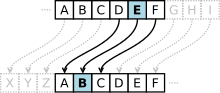
\includegraphics[width=\linewidth]{fig/Caesar_cipher_left_shift_of_3.svg.png}
        \captionof{figure}{Ceasar cipher}
        \end{minipage}
        
        \hfill
        
        \begin{minipage}{0.49\linewidth}
        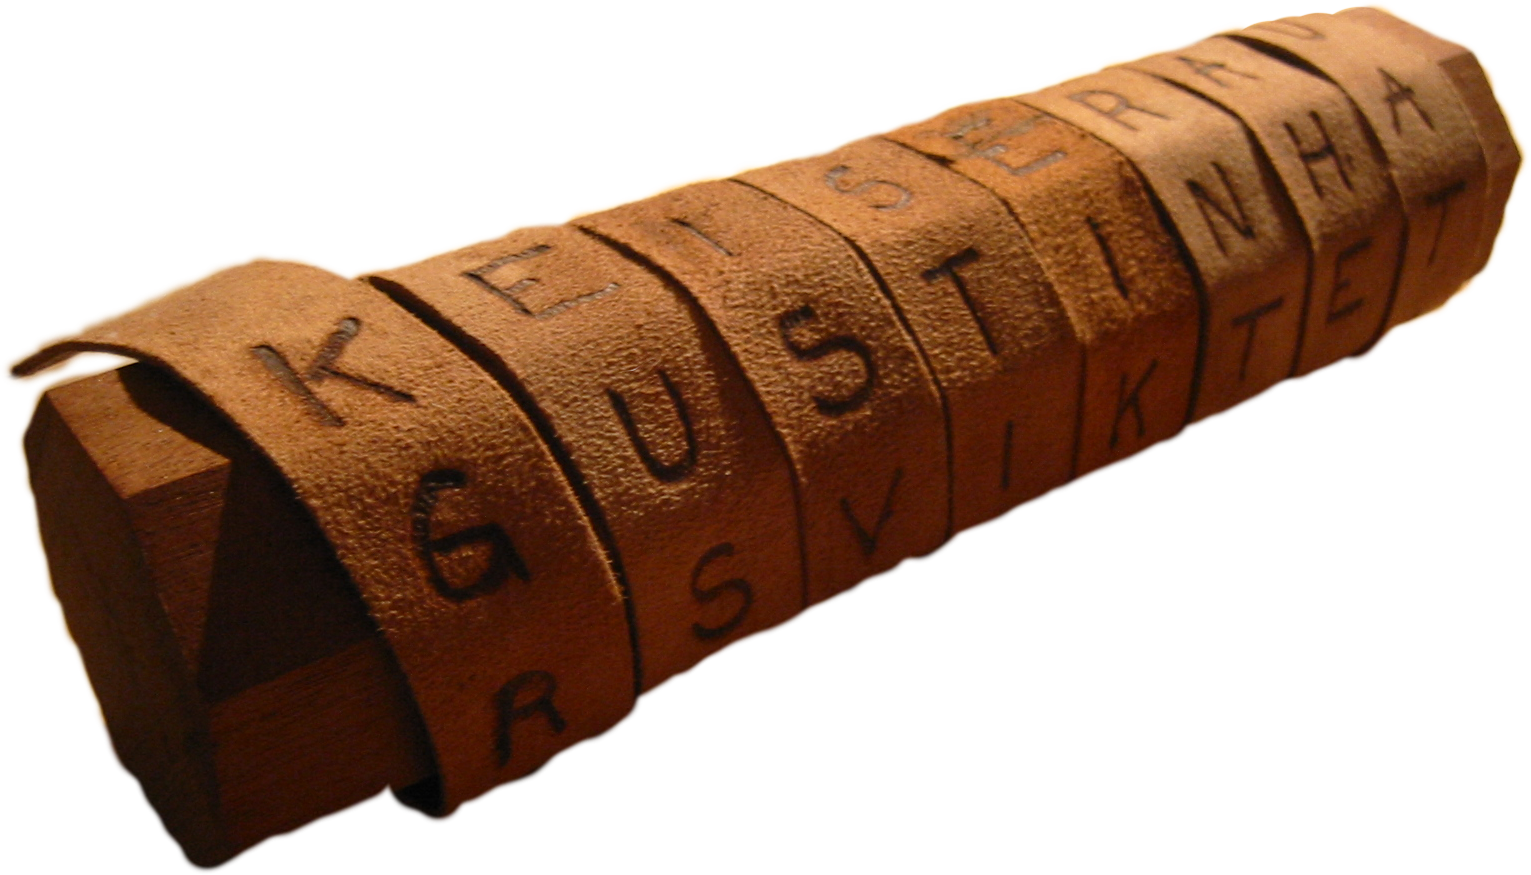
\includegraphics[width=\linewidth]{fig/Skytale.png}
        \captionof{figure}{Skytale}
        \end{minipage}
        
        \captionof{figure}{Examples of ancient cryptographic machinery}
    \end{center}
\end{frame}

\begin{frame}{First cryptographers}
    \begin{center}
        \begin{minipage}{0.45\linewidth}
            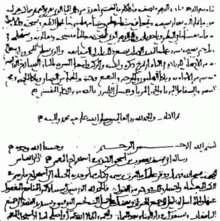
\includegraphics[width=\linewidth]{fig/Al-kindi_cryptographic.png}
            \captionof{figure}{The first page of al-Kindi's manuscript ''On Deciphering Cryptographic Messages'', 
        containing the oldest known description of cryptanalysis by frequency analysis.}
        \end{minipage}
        \hfill
        \begin{minipage}{0.45\linewidth}
            \begin{center}
                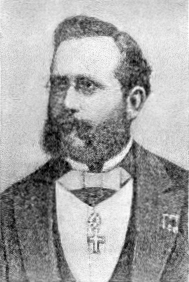
\includegraphics[width=0.4\linewidth]{fig/Auguste_Kerckhoffs.jpg}
                \captionof{figure}{Auguste Kerckhoffs}
                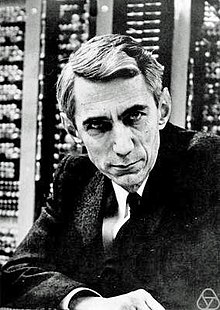
\includegraphics[width=0.4\linewidth]{fig/220px-ClaudeShannon_MFO3807.jpg}
                \captionof{figure}{Claude Shannon}
            \end{center}
        \end{minipage}            
    \end{center}
\end{frame}

\begin{frame}{Modern cryptography}
    \begin{center}
    \begin{minipage}{0.45\linewidth}
        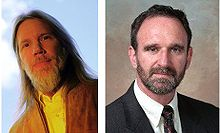
\includegraphics[width=0.7\linewidth]{fig/220px-Diffie_and_Hellman.jpg}
        \captionof{figure}{Whitfield Diffie and Martin Hellman, authors of the first published paper on public-key 
        cryptography.}
    \end{minipage}
    \hfill
    \begin{minipage}{0.5\linewidth}
        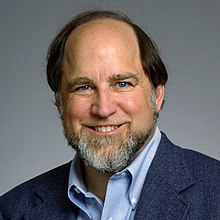
\includegraphics[width=0.3\linewidth]{fig/Ronald_L_Rivest_photo.jpg}
        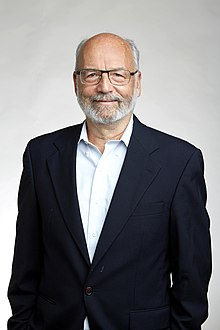
\includegraphics[width=0.33\linewidth]{fig/Adi_Shamir_Royal_Society.jpg}
        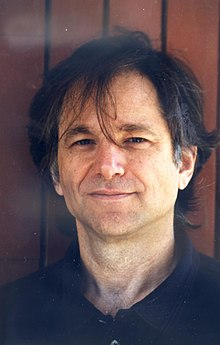
\includegraphics[width=0.33\linewidth]{fig/Len-mankin-pic.jpg}
        \captionof{figure}{Ron Rivest, Adi Shamir and Leonard Adleman --- reinventors of RSA cryptosystem.}
    \end{minipage}
    \end{center}
\end{frame}

\begin{frame}{Applications of cryptography}
    \subsection{Applications of cryptography}
    \begin{itemize}
        \item Blockchains
        \item Secure messaging
        \item SSL$\backslash$TLS
        \item Secure data storage
        \item You name it!
    \end{itemize}
\end{frame}

\begin{frame}{Why mathematical cryptography?}
    \subsection{Mathematical cryptography}
    Selected topics in mathematics
    \begin{itemize}
        \item Abstract algebra (must have!)
        \item Number theory (must have!) --- although we will only scratch the surface
        \item Probability theory
        \item Category theory
    \end{itemize}
\end{frame}

%%%%%%%%%%%%%%%%%%%%%%%%%%%%%%%%%%%%%%%%%%%%%%%%%%%%%%%%%%%

\begin{frame}{Basic Abstract Algebra}
    \section{Basic Abstract Algebra}
    \subsection{Preliminaries}
    Sets (later we will define more rigorous terms) we are going to extensively use:
    \begin{itemize}
        \item $\mathbb{N}$, $\mathbb{Z}$
        \item $\mathbb{Z} / n\mathbb{Z}$ --- the set of integers modulo n
        \item $\mathbb{Z} / n \mathbb{Z}^{*}$ --- important set that we will define later in this lecture
    \end{itemize} 
\end{frame}

\begin{frame}{Functions (mappings)}
    \subsection{Functions}
    \begin{definition}
        A function from set $X$ (domain) to set $Y$ (co-domain) is an assignment of an element of $Y$ to each element
        of $X$. A function is called to be 'well-defined' if and only if for each element from domain there exists 
        exactly one element from co-domain.  
    \end{definition}
    \begin{example}
        An example of not well-defined function: \\
        \begin{align*}
            & \varphi : \mathbb{Q} \to \mathbb{Z} \\
            & \varphi : \frac{p}{q} \mapsto p \cdot q \\
            & \varphi\left(\frac{2}{4}\right) = 8 \ne \varphi\left(\frac{1}{2}\right) = 2
        \end{align*}
    \end{example}
\end{frame}

\begin{frame}{Image and preimage of a function}
    \begin{definition}
        Image of a function is a set of all output values it can produce. \\
        Formally
        \begin{eqnarray*}
            & \psi : X \to Y, A \subseteq X \\
            & \psi[A] = \left\{\psi(a) : a \in A \right\} = B, B \subseteq Y
        \end{eqnarray*}
    \end{definition}
    \begin{definition}
        Preimage of a function is a set of all values that produce the given outputs.
        Formally
        \begin{equation*}
            \psi^{-1}[B] = \left\{x \in X : \psi(x) \in B \right\} = A
        \end{equation*}
    \end{definition}
\end{frame}

\begin{frame}{Surjection, injection and bijection}
    \begin{center}
        \begin{minipage}{0.48\linewidth}
            \centering
            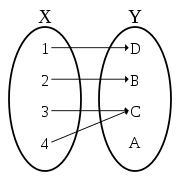
\includegraphics[width=0.5\linewidth]{fig/180px-Not-Injection-Surjection.svg.png}
            \captionof*{figure}{neither injection nor surjection}
            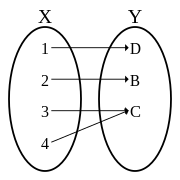
\includegraphics[width=0.49\linewidth]{fig/Surjection.svg.png}
            \captionof*{figure}{surjection}

        \end{minipage}
        \hfill
        \begin{minipage}{0.49\linewidth}
            \centering
            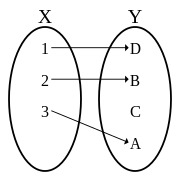
\includegraphics[width=0.5\linewidth]{fig/Injection.svg.png}
            \captionof*{figure}{injection}
            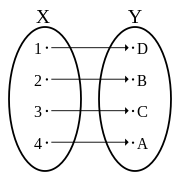
\includegraphics[width=0.5\linewidth]{fig/Bijection.svg.png}
            \captionof*{figure}{bijection}
        \end{minipage}
    \end{center}
\end{frame}

\begin{frame}{Basic properties of integers}
    \section{Basic properties of integers}
    \subsection{Integer divisibility}
    \begin{definition}
        $a \mid b$ - $a$ divides $b$
        \begin{eqnarray*}
                & a, b \in \mathbb{Z} & \\
                & a \mid b \iff \exists(!) c \in \mathbb{Z} : b = c \cdot c
        \end{eqnarray*}
        (!) Only in $\mathbb{Z}$ and other PIDs (PIDs are not covered in this course) 
    \end{definition}
    \begin{definition}
        An integer is called prime, iff it has only 2 divisors: 1 and itself
    \end{definition}
    \begin{definition}
        An integer is called composite if it has more than 2 distinct divisors
    \end{definition}
\end{frame}

\begin{frame}{GCD and LCM}
    \begin{definition}
        GCD --- Greatest Common Divisor \\
        $\gcd(a, b) (\text{or just (a, b)})= \max \left\{ c \in \mathbb{Z} : c \mid a \text{ and } c \mid b \right\}$
    \end{definition}
    \begin{example}
        $ \gcd(12, 4) = 4, \quad \gcd(64, 12) = 4 $ 
    \end{example}

    \begin{definition}
        LCM --- Least Common Multiple \\
        $\text{lcm}(a, b) = \min \left\{ c \in \mathbb{Z}_{> 0} : a \mid c \text{ and } b \mid c \right\}$
    \end{definition}
    \begin{example}
        $ \text{lcm}(12, 4) = 12, \quad \text{lcm}(64, 12) = 192 $
    \end{example}

\end{frame}

\begin{frame}{Fermat's little theorem}
    \subsection{Fermat's little theorem}
    \begin{Theorem}[Fermat's little theorem]
        $p$ --- prime, $a \in \mathbb{Z}$ \\
        $a^p \equiv a \pmod p$
    \end{Theorem}
    \begin{example}
        $ 2^7 \equiv 2 \pmod 2, \quad -1^{13} \equiv 12 \pmod {13} $
    \end{example}
    Proof: on the next lecture
\end{frame}

\begin{frame}{Euler's totient function and Euler's theorem}
    \subsection{Euler's totient function and Euler's theorem}
    \begin{definition}
        $\varphi(n)$ --- The number of positive integers less than $n$ s.t. they are coprime.
        Formally:
        \begin{equation*}
            \varphi(n) = \# \left\{ x : (x, n) = 1 \right\}
        \end{equation*} 
    \end{definition}
    \begin{Theorem}[Euler's theorem]
        \begin{eqnarray*}
            & a \in \mathbb{Z}, n \in \mathbb{Z}_{>0} \\
            & a^{\varphi(n)} \equiv a \pmod n
        \end{eqnarray*}
    \end{Theorem}
    In other words: it is more general version of Fermat's little theorem. \\
    Both Euler's phi function and Euler's theorem are essential for understanding the RSA cryptosystem.
\end{frame}

\begin{frame}{Introduction to SageMath}
    \section{Introduction to SageMath}
    \begin{itemize}
        \item Download and install SageMath from \\ \url{https://doc.sagemath.org/html/en/installation/index.html}
        \item Or, alternatively, use \\ \url{https://sagecell.sagemath.org/} for online access.
    \end{itemize}
\end{frame}

\begin{frame}{Homework}
    \section{Homework}
    Build an bijection $\varphi : \mathbb{Z} \to \mathbb{N}_{>0}$ and show that $\varphi$ is indeed a bijection. \\ 
    Hint: show that $\varphi$ is the surjection and injection simultaneously.
\end{frame}

\begin{frame}{Next lecture}
    \section{Next lecture topic}
    On the next lecture we are going to dig deep into Abstract Algebra, and learn new mathematical objects, such as 
    semigroups, monoids and groups, as well as prove the Fermat's \st{last} little theorem and Euler's theorem.
\end{frame}

\end{document}
